\documentclass{anstrans}
%%%%%%%%%%%%%%%%%%%%%%%%%%%%%%%%%%%
\title{Boundary Conditions for the Anisotropic Diffusion Approximation}
\author{Seth R.~Johnson \and Edward W.~Larsen}

\institute{Department of Nuclear Engineering \& Radiological Sciences, University of Michigan, Ann Arbor, MI, 48109}
\email{sethrj@umich.edu \and edlarsen@umich.edu}
\usepackage{amssymb}
\usepackage{microtype}
\usepackage{graphicx}
\usepackage{booktabs} % \toprule, \midrule, \bottomrule
%%% INCLUDE FILE FOR DEFINITIONS
%%% These may require various packages.

% Shortcuts in regular text
\newcommand{\degs}{\ensuremath{^\circ}}
\newcommand{\EE}[1]{\ensuremath{\times 10^{#1}}}
\newcommand{\ttimes}{\ensuremath{{}\times{}}}
\newcommand{\cclicense}{%
  \smash{\raisebox{-0.45ex}{%
  \setlength{\unitlength}{1em}%
  \begin{picture}(1,1)%
    \put(0.5,0.5){\circle{1}}
    \put(0.5,0.5){\hbox to 0pt{\hss\raisebox{-.45ex}{\tiny\textsf{CC}}\hss}}
  \end{picture}%
  }}%
  \hskip -1em%
  \href{http://creativecommons.org/licenses/by-nc-sa/3.0/}%
  {\ \hskip 1em \textsf{BY-NC-SA}}%
}

%\newcommand{\horizsep}{{\par\noindent\centering\rule[.25ex]{.75\columnwidth}{2pt}\par}}
\newcommand{\horizsep}{\vspace{\baselineskip}\noindent\hspace{\stretch{1}}$
\ast\qquad \ast\qquad \ast\qquad
$ \hspace{\stretch{1}} \vspace{\baselineskip}}
\newcommand{\pytrt}{\textsf{PyTRT}}

% Research
\newcommand{\lop}[1]{\mathcal{L}\!\left[#1\right]}
\newcommand{\lopinv}[2]{\mathcal{I}_{#1}\!\left[#2\right]}
\newcommand{\Dtens}{\mat{D}}
\newcommand{\Etens}{\mat{E}}
\newcommand{\Identitytens}{\mat{I}}
\newcommand{\APone}{AP$_1$}
\newcommand{\Pone}{P$_1$}
\newcommand{\SN}{S$_N$}%{S$_\text{N}$}%{$S_N$}%
\newcommand{\PN}{P$_N$}%{P$_\text{N}$}%{$P_N$}%
\newcommand{\CN}{Crank--Nicolson} %Yes, it's Nic not Nich
\newcommand{\Eddington}{\mathcal{E}} %whatever symbol I decided for Eddington
\newcommand{\RadEn}{E} %whatever symbol I decide for radiation energy
\newcommand{\Sigmatr}{\Sigma_{\mathit{tr}}}

% Program names
\newcommand{\cpp}{\textsf{C\raisebox{0.2ex}{++}}}

% General math shortcuts
\newcommand{\ud}{\mathop{}\!\mathrm{d}}
\newcommand{\pder}[2]{\frac{\partial #1}{\partial #2}}
\newcommand{\oder}[2]{\frac{\mathrm{d} #1}{\mathrm{d} #2}}
\newcommand{\tpder}[2]{{\partial #1}/{\partial #2}} %inlined
\newcommand{\toder}[2]{{\mathrm{d} #1}/{\mathrm{d} #2}} %inlined
\newcommand{\lra}{ \quad \Longrightarrow \quad }
\newcommand{\eexp}{\mathop{}\!\mathrm{e}} % upright ``e'' for exponent
\newcommand{\expp}[1]{\exp\!\left( {#1} \right)} % exp with parentheses
\newcommand{\qeq}{\stackrel{\mathrm{?}}{=}}

% Probability
\newcommand{\expectation}[1]{\mathop{}\!\mathrm{E}\!\left[ #1 \right]}
\DeclareMathOperator{\Var}{Var} % variance

% Asymptotic analysis
\DeclareMathOperator{\Ei}{Ei} % Exponential function
\newcommand{\lapl}[1]{\mathcal{L}[{#1}]} %laplace

%change the Re and Im operators from fancy curly letters
\DeclareMathOperator{\MathOpRe}{Re}
\renewcommand{\Re}{\MathOpRe}
\DeclareMathOperator{\MathOpIm}{Im}
\renewcommand{\Im}{\MathOpIm}

%imaginary ``i'' , upright 'i' or \imath
\newcommand{\iimag}{\mathrm{i}}

% Finite differences
\newcommand{\hot}{\text{h.o.t.}}
\newcommand{\inv}{^{-1}}

% Numerical Linear Algebra
\newcommand{\conj}{^{\ast}} % complex conjugate (transpose)
\newcommand{\norm}[1]{\left\| #1 \right\|} % double pipe
\newcommand{\abs}[1]{\left| #1 \right|} % single pipe
\newcommand{\eps}{\varepsilon}
\DeclareMathOperator{\fl}{fl}

\DeclareMathOperator{\acosh}{arccosh} 

% Define a command to write a nice-looking element, e.g. 4,2 He
\newcommand{\elem}[3]{\ensuremath{{}^{{#1}}_{{#2}}\mathrm{{#3}}}}

% Vector definitions
\newcommand{\mat}[1]{\mathbf{#1}} %matrix is bold upright
\renewcommand{\vec}[1]{\bm{#1}} %vector is bold italic
\newcommand{\op}[1]{\mathsf{#1}} % ``operator'' is sans serif

\newcommand{\vd}{\bm{\cdot}} % slightly bold vector dot
\newcommand{\del}{\vec{\nabla}} % gradient (Del) is bold
\newcommand{\grad}{\vec{\nabla}} % gradient

%\newcommand{\abr}[1]{\langle {#1} \rangle}
\newcommand{\abr}[1]{\left\langle {#1} \right\rangle} % angle brackets for avg.

%% topbox is useful in extended definitions of math terms inside an align
\newcommand{\topbox}[2][0.6]{\parbox[t]{#1\columnwidth}{\raggedright{}#2}}

% commands to make text in math mode appear as zero-width (better-looking
% integrals/sums, e.g.)
% from mathmode.pdf page 74, or Alexander R. Perlis ``A complement to \smash,
% \llap, and \rlap''

\def\mathllap{\mathpalette\mathllapinternal}
	\def\mathllapinternal#1#2{%
	\llap{$\mathsurround=0pt#1{#2}$}%
}
\def\clap#1{\hbox to 0pt{\hss#1\hss}}%
\def\mathclap{\mathpalette\mathclapinternal}%
\def\mathclapinternal#1#2{%
	\clap{$\mathsurround=0pt#1{#2}$}%
}
\def\mathrlap{\mathpalette\mathrlapinternal}%
\def\mathrlapinternal#1#2{%
	\rlap{$\mathsurround=0pt#1{#2}$}%
}

\newcommand{\url}[1]{\texttt{#1}}

% graphics paths
\graphicspath{{/Users/seth/_research/figures/}}
\makeatletter
\def\input@path{{/Users/seth/_research/figures/}}
\makeatother

\renewcommand{\bottomfraction}{1.}
\renewcommand{\topfraction}{1.}

\hyphenpenalty=800
\tolerance=400

%\usepackage{setspace}
%\doublespacing

%\AtBeginDocument{\setlength{\baselineskip}{11pt}}
\setlength{\parskip}{0pt}

\begin{document}
%%%%%%%%%%%%%%%%%%%%%%%%%%%%%%%%%%%%%%%%%%%%%%%%%%%%%%%%%%%%%%%%%%%%%%%%%%%%%%%%
\section{Introduction}
Recently, an anisotropic diffusion (AD) equation has been derived that uses
transport-calculated AD coefficients to inexpensively but accurately model
particle transport, particularly in voided channels where standard diffusion
theory breaks down \cite{Lar2009c,Joh2011,Tra2011}. However, these derivations
of the AD equation did not address boundary conditions:\ numerical simulations
to test the equations used heuristic boundary conditions.

Here we present a new derivation of the AD approximation in which the AD
equation and boundary conditions are both obtained systematically. Also, we
numerically test the AD equation and the proposed boundary conditions on a
``flatland" VHTR-like problem driven by a boundary source, and we demonstrate
that the results are highly accurate. 

%%%%%%%%%%%%%%%%%%%%%%%%%%%%%%%%%%%%%%%%%%%%%%%%%%%%%%%%%%%%%%%%%%%%%%%%%%%%%%%%
\section{Derivation}
We consider a 3D, monoenergetic, steady-state transport equation
with isotropic scattering and an isotropic source:
\begin{subequations} \label{eqs:fullTransport}
\begin{multline} 
  \vec{\Omega}\vd \grad \psi(\vec{x}, \vec{\Omega})
  + \sigma(\vec{x}) \psi (\vec{x}, \vec{\Omega})
  = \frac{\sigma_s(\vec{x})}{4\pi} \int_{4\pi} \psi(\vec{x},\vec{\Omega}')
    \ud\Omega' 
 \\ 
  {}+ \frac{q(\vec{x})}{4\pi} 
  \equiv \frac{1}{4\pi} Q(\vec{x}) \,, \quad
    \vec{x} \in V, \; \vec{\Omega} \in 4\pi \,,
    \label{eq:fullTransportVol}
\end{multline}
with an incident flux boundary condition
\begin{equation} \label{eq:fullTransportBndy}
  \psi(\vec{x}, \vec{\Omega}) = \psi^b(\vec{x}, \vec{\Omega}) \,,
 \quad \vec{x} \in \partial V, \ \vec{\Omega} \vd \vec{n} < 0\,.
\end{equation}
\end{subequations}

Operating on Eq.~\eqref{eq:fullTransportVol} by $\int_{4\pi} (\cdot) \ud
\Omega$ gives the particle conservation equation
\begin{equation} \label{eq:loVol}
  \grad \vd\vec{J}(\vec{x})
  + \sigma(\vec{x}) \phi(\vec{x})
  = Q(\vec{x})\,,
  \quad \vec{x} \in V\,.
\end{equation}
Adding $\vec{\Omega}\vd \grad \phi$ to both sides of Eq.~\eqref{eq:loVol},
dividing the result by $4\pi$, and subtracting from
Eq.~\eqref{eq:fullTransportVol}, the isotropic scattering and extraneous
sources cancel.
%\begin{equation*}
%  \vec{\Omega}\vd \grad \left[ \psi
%  - \tfrac{1}{4\pi} \phi \right]
%  + \sigma \left[ \psi
%  - \tfrac{1}{4\pi} \phi \right]
%  = 0 + \tfrac{1}{4\pi} \grad \vd\vec{J} -
%  \tfrac{1}{4\pi} \vec{\Omega}\vd \grad \phi\,.
%\end{equation*}
Then, defining 
%\begin{equation}\label{eq:capPsi}
$  \Psi(\vec{x},\vec{\Omega}) \equiv \psi(\vec{x},\vec{\Omega})
  - \tfrac{1}{4\pi} \phi(\vec{x})\,, $
%\end{equation}
we get
\begin{subequations} \label{eqs:capPsiTransport}
\begin{equation} \label{eq:capPsiVol}
  \vec{\Omega}\vd \grad \Psi(\vec{x}, \vec{\Omega})
  + \sigma(\vec{x}) \Psi(\vec{x}, \vec{\Omega})
  = \tfrac{1}{4\pi} \grad \vd\vec{J}(\vec{x}) -
  \tfrac{1}{4\pi} \vec{\Omega}\vd \grad \phi(\vec{x})\,.
\end{equation}
Subtracting $\phi/4\pi$ from Eq.~\eqref{eq:fullTransportBndy} gives the
boundary condition
\begin{equation}\label{eq:capPsiBndy}
 \Psi(\vec{x}, \vec{\Omega}) 
  =\psi^b(\vec{x}, \vec{\Omega}) - \tfrac{1}{4\pi} \phi(\vec{x})\,,
  \quad \vec{x} \in \partial V,\ \vec{\Omega} \vd \vec{n} < 0\,.
\end{equation}
\end{subequations}
The transport solution $\psi$ satisfies these equations exactly. Also,
$\Psi$ satisfies the identities
\begin{equation} \label{eq:capPsiIdentities}
  \int_{4\pi} \Psi(\vec{x}, \vec{\Omega}) \ud\Omega = 0
  \quad\text{and}\quad
  \int_{4\pi} \vec{\Omega}\Psi(\vec{x}, \vec{\Omega}) \ud\Omega =
  \vec{J}(\vec{x})\,.
\end{equation}

% Introducing the linear-in-angle approximation $\Psi\approx \frac{3}{4\pi}
% \vec{\Omega}\vd\vec{J}$ into Eq.~\eqref{eq:capPsiVol} and taking the first
% angular moment would yield Fick's law, but the AD method does something far
% stranger.

%In order to formulate transport-matched boundary conditions, 
To proceed, we write $\Psi$ as the sum of
an ``interior" solution $\tilde\Psi$ and a ``boundary layer" solution
$\Psi_\mathrm{bl}$:
\begin{equation} \label{eq:boundaryLayerPsi}
  \Psi(\vec{x}, \vec{\Omega})
  = \tilde\Psi(\vec{x}, \vec{\Omega})
  + \Psi_\mathrm{bl}(\vec{x}, \vec{\Omega})\,.
\end{equation}
The interior transport equation is just like Eq.~\eqref{eq:capPsiVol}:
\begin{subequations} \label{eqs:tCapPsi}
\begin{equation} \label{eq:tCapPsiVol}
  \vec{\Omega}\vd \grad \tilde\Psi(\vec{x}, \vec{\Omega})
  + \sigma(\vec{x}) \tilde\Psi(\vec{x}, \vec{\Omega})
  = \frac{1}{4\pi} \grad \vd\vec{J}(\vec{x}) -
  \frac{1}{4\pi} \vec{\Omega}\vd \grad \phi(\vec{x})\,.
\end{equation}
We define incident boundary conditions for this interior solution
to be
\begin{equation}\label{eq:tCapPsiBndy}
 \tilde\Psi(\vec{x}, \vec{\Omega}) 
  = - \zeta(\vec{x}, \vec{\Omega}) \vec{\Omega}\vd \grad \phi(\vec{x})
  \equiv \tilde\Psi^b(\vec{x}, \vec{\Omega}) \,,
\end{equation}
\end{subequations}
where $\zeta$ is a to-be-determined function on the boundary.
The boundary layer solution complements the interior solution, but is expected
to tend to zero rapidly with distance from the outer boundary. Its transport
equation has no internal source, and its boundary condition is
Eq.~\eqref{eq:tCapPsiBndy} subtracted from Eq.~\eqref{eq:capPsiBndy}:
\begin{equation} \label{eq:blCapPsiBndy}
 \Psi_\mathrm{bl}(\vec{x}, \vec{\Omega}) 
  = \psi^b(\vec{x}, \vec{\Omega}) - \frac{1}{4\pi} \phi(\vec{x})
  + \zeta(\vec{x}, \vec{\Omega}) \vec{\Omega}\vd \grad \phi(\vec{x})\,.
\end{equation}

Integrating along a characteristic ray transforms the differential
equation~\eqref{eq:tCapPsiVol} and its boundary condition~\eqref{eq:tCapPsiBndy}
into an integral transport equation
\cite{Pri2010}:
\begin{subequations} \label{eqs:inverseTransport}
\begin{align} \label{eq:inverseTransportFull}
\begin{split}
  \tilde\Psi(\vec{x}, \vec{\Omega})
  &=
  \tilde\Psi^b(\vec{x} - s_b\vec{\Omega}, \vec{\Omega})
  \eexp^{ -\tau(\vec{x}, \vec{x} - s_b \vec{\Omega})}
  \\
  &\quad +  \int_{0}^{s_b}
  \Big[\tfrac{1}{4\pi} \grad \vd\vec{J}(\vec{x} - s \vec{\Omega}, \vec{\Omega})
  \\
  &\quad\qquad - \tfrac{1}{4\pi} \vec{\Omega}\vd \grad \phi(\vec{x} - s
  \vec{\Omega}, \vec{\Omega}) \Big]
  \eexp^{ -\tau(\vec{x}, \vec{x} - s \vec{\Omega})} \ud s
\end{split}
\\ \label{eq:inverseTransportBrief}
\begin{split}
%  \tilde\Psi(\vec{x}, \vec{\Omega})
    &\equiv
    -\lopinv{b}{\zeta \vec{\Omega}\vd \grad \phi}
    + \lopinv{v}{\tfrac{1}{4\pi} \grad \vd\vec{J} }
    - \lopinv{v}{\tfrac{1}{4\pi} \vec{\Omega}\vd \grad \phi}\,.
\end{split}
\end{align}
\end{subequations}
Here $\tau(\vec{x}, \vec{x}')$ is the optical thickness of the medium between
points
$\vec{x}$ and $\vec{x}'$
along the direction $\vec{\Omega} = (\vec{x}'-
\vec{x})/\norm{\vec{x}'-\vec{x}}$,
and $s_b$ is the distance to the boundary along $-\vec{\Omega}$ from
$\vec{x}$.

Now we assume that the spatial gradients of the angular flux
are weak, and the solution is mildly (but not necessarily linearly) anisotropic:
\begin{align} \label{eq:ansatz}
  \psi &= O(1), &
  \grad \psi &= O(\epsilon), &
  \int_{4\pi} \vec{\Omega} \psi\ud\Omega &= O(\epsilon).
\end{align}
Then $\grad \vd\vec{J}=O(\epsilon^2)$, and the second term in
Eq.~\eqref{eq:inverseTransportBrief} is neglected.
We also expand the nonlocal variables in Eq.~\eqref{eq:inverseTransportFull}
about the local spatial point:
\begin{equation} \label{eq:taylorPhi}
  \phi(\vec{x} - s \vec{\Omega})
  \sim \phi(\vec{x}) - s \vec{\Omega} \vd \grad \phi (\vec{x}) + O(\epsilon^2)
  \sim \phi(\vec{x}) + O(\epsilon) \,.
\end{equation}
Then the third term in Eq.~\eqref{eq:inverseTransportBrief} simplifies to
\begin{align}\nonumber
- \lopinv{v}{\frac{1}{4\pi} \vec{\Omega}\vd \grad \phi(\vec{x})}
  &\approx \int_{0}^{\norm{\vec{x} - \vec{x}_b}}
    \left[ -\frac1{4\pi}\vec{\Omega}\vd \grad \phi(\vec{x}) \right]
    \eexp^{ -\tau(\vec{x}, \vec{x} - s \vec{\Omega})}
    \ud s
  \\\nonumber
  &= - \int_{0}^{\norm{\vec{x} - \vec{x}_b}}
    \left[ \tfrac1{4\pi}\right]
    \eexp^{ -\tau(\vec{x}, \vec{x} - s \vec{\Omega})} \ud s \,
    \vec{\Omega}\vd \grad \phi(\vec{x})
  \\\label{eq:streamingApprox}
  &= - \lopinv{v}{ \tfrac1{4\pi} } \vec{\Omega}\vd \grad \phi(\vec{x}) +
  O(\epsilon^2) \,.
\end{align}
Similarly, the boundary term in Eq.~\eqref{eq:inverseTransportBrief} becomes
\begin{equation} \label{eq:bndyApprox}
-\lopinv{b}{\zeta \vec{\Omega}\vd \grad \phi}_{\partial V_b}
\approx -\lopinv{b}{\zeta}_{\partial V_b} \vec{\Omega}\vd \grad \phi(\vec{x})
+ O(\epsilon^2) \,.
\end{equation}
Substituting Eqs.~\eqref{eq:streamingApprox} and~\eqref{eq:bndyApprox} into
Eq.~\eqref{eq:inverseTransportBrief}, and discarding $O(\epsilon^2)$ terms, we
obtain
\begin{align} \label{eq:approxPsi2}
  \tilde\Psi(\vec{x}, \vec{\Omega}) 
  &\approx 
- \lopinv{b}{\zeta}_{\partial V_b} \vec{\Omega}\vd \grad \phi
- \lopinv{v}{\tfrac{1}{4\pi}}  \vec{\Omega}\vd \grad \phi
%\\ \label{eq:approxPsi2}
%  \tilde\Psi &= 
%- \left\{ \lopinv{b}{\zeta}_{\partial V_b} 
%+ \lopinv{b}{f(\vec{\Omega}_r)}_{\partial V_r}
%+ \lopinv{v}{\frac{1}{4\pi}} \right\} \vec{\Omega}\vd \grad \phi
\nonumber \\ %\label{eq:approxPsi3}
   &\equiv - f(\vec{x}, \vec{\Omega})
\vec{\Omega}\vd \grad \phi(\vec{x})\,.
\end{align}
Converting the $\lopinv{}{\cdot}$ terms back into the differential form, we
find that $f$ satisfies a purely absorbing transport equation with a
uniform, unit isotropic source:
\begin{subequations} \label{eqs:fFull}
  \begin{equation} \label{eq:fFullVol}
    \vec{\Omega}\vd \grad f(\vec{x}, \vec{\Omega})
    + \sigma(\vec{x}) f (\vec{x}, \vec{\Omega})
  = \tfrac{1}{4\pi} \,, \quad x \in V,\ \vec{\Omega} \in 4\pi\,,
  \end{equation}
with a to-be-determined boundary condition:
\begin{equation} \label{eq:fFullBndy}
  f(\vec{x}, \vec{\Omega}) = \zeta(\vec{x}, \vec{\Omega}) \,,
 \quad \vec{x} \in \partial V, \ \vec{\Omega} \vd \vec{n} < 0\,.
\end{equation}
\end{subequations}

We use the identity from Eq.~\eqref{eq:capPsiIdentities} to get an expression
for the current by taking the first moment of Eq.~\eqref{eq:approxPsi2}:
\begin{align} \nonumber
  \vec{J}(\vec{x})
  &= 
  - \left( \int_{4\pi} \vec{\Omega} \vec{\Omega} f(\vec{x}, \vec{\Omega})
  \ud\Omega \right)
  \vd \grad \phi(\vec{x})
  \\ \label{eq:anisotropicFicks}
  &= - \Dtens(\vec{x}) \vd \grad \phi(\vec{x}) \,.
\end{align}
This resembles Fick's law, but instead of a scalar diffusion coefficient,
the anisotropic diffusion method has a diffusion \emph{tensor}, $\Dtens$, the
second angular moment of $f$.

The unknown function $\zeta(\vec{x}, \vec{\Omega})$, introduced at the
beginning of the anisotropic
diffusion derivation, allowed us to formulate a specified boundary condition
such that the effect of $\zeta$ could be embedded in the anisotropic diffusion
tensor $\Dtens$. To make use of this degree of freedom, we enforce on
the boundary the fact from Eq.~\eqref{eq:capPsiIdentities} that the zeroth
moment of $\Psi(\vec{x}, \vec{\Omega})$ is zero. Applying the identity to
Eq.~\eqref{eq:approxPsi2} shows that for this to hold, we must have
\begin{equation}\label{eq:zetaCondition}
  \int_{\vec{\Omega}\vd \vec{n} > 0}\vec{\Omega}
  f(\vec{x},\vec{\Omega}) \ud\Omega
  =
  \int_{\vec{\Omega}\vd \vec{n} < 0}(-\vec{\Omega}) \zeta(\vec{x},\vec{\Omega})
  \ud\Omega \,.
\end{equation}
One way to satisfy this is to make $f$ an even function of $\vec{\Omega}$,
$\zeta(\vec{\Omega})=f(-\vec{\Omega})$. Furthermore, if
$f$ is azimuthally symmetric about $\vec{n}$ on the boundary, then
\begin{equation*}
f(\vec{x}, \vec{\Omega}) = \zeta(\vec{x},\vec{\Omega})
  = f(\vec{x},\vec{\Omega}-2(\vec{n}\vd\vec{\Omega})\vec{n})\,,
 \quad \vec{x} \in \partial V, \ \vec{\Omega} \vd \vec{n} < 0\,,
\end{equation*}
which is a specular reflecting boundary condition for $f$.

Now we return to the boundary layer transport equation~\eqref{eq:blCapPsiBndy}.
A lengthy analysis shows that the transport boundary layer decays most rapidly
if the solution of the approximate method satisfies the boundary condition
\begin{equation} \label{eq:bcW}
  0 = \int_{\vec{\Omega} \vd \vec{n} < 0} W(\abs{\vec{\Omega} \vd \vec{n}})
  \Psi_\mathrm{bl} (\vec{x}, \vec{\Omega}) \ud \Omega\,,\qquad \vec{x} \in
  \partial V\,,
\end{equation}
where $W(\mu)$ is well approximated by the simple polynomial $\mu +
\tfrac{3}{2} \mu^2$ \cite{Mal1991}. 
Applying Eq.~\eqref{eq:bcW} to Eq.~\eqref{eq:blCapPsiBndy}, we find
\begin{multline*}
  2\int_{\vec{\Omega}\vd \vec{n} < 0}
  W(\abs{\vec{\Omega} \vd \vec{n}}) \psi^b(\vec{x}, \vec{\Omega}) \ud\Omega
 \\  = \phi(\vec{x})
 - 2\int_{\vec{\Omega}\vd \vec{n} < 0} W(\abs{\vec{\Omega} \vd \vec{n}})
  \zeta(\vec{x}, \vec{\Omega}) \vec{\Omega} \ud\Omega
  \vd \grad \phi(\vec{x})\,,
\end{multline*}
or, rewriting the right hand side in terms of incident angles using
$\zeta(\vec{\Omega})= f(-\vec{\Omega})$,
\begin{multline}\label{eq:loBndy}
  2\int_{\vec{\Omega}\vd \vec{n} < 0}
  W(\abs{\vec{\Omega} \vd \vec{n}}) \psi^b(\vec{x}, \vec{\Omega}) \ud\Omega
 \\ = \phi(\vec{x})
  + 2\int_{\vec{\Omega}\vd \vec{n} > 0} W(\vec{\Omega} \vd \vec{n})
  \vec{\Omega} f(\vec{x}, \vec{\Omega}) \ud\Omega
  \vd \grad \phi(\vec{x}) \,.
\end{multline}
If instead we use $W(\mu)=2\mu$, we obtain a less accurate Marshak-like
boundary condition
\begin{equation}\label{eq:marshakAd}
  4 J^-(\vec{x})
  = \phi(\vec{x})
  + 2 \vec{n} \vd \Dtens(\vec{x}) \vd \grad \phi(\vec{x}) \,,
\end{equation}
where $J^- \equiv \int_{\vec{\Omega}\vd \vec{n} < 0} \abs{\vec{\Omega} \vd
\vec{n}} \psi^b \ud\Omega$ is the incident current.

%%%%%%%%%%%%%%%%%%%%%%%%%%%%%%%%%%%%%%%%%%%%%%%%%%%%%%%%%%%%%%%%%%%%%%%%%%%%%%%%
\section{Discussion}
%The invention of $\zeta$ allows $\Dtens$ to account for boundary effects. It
%results in a
%boundary condition both for $f$ and for the low-order problem that calculates
%$\phi$.

In a homogeneous medium, the reflecting boundary condition on $f$ gives a
solution
$f=1/(4\pi\sigma)$, which gives the standard diffusion result $\Dtens=
\Identitytens/(3\sigma)$ and causes Eq.~\eqref{eq:loBndy} to simplify to
the transport-corrected diffusion boundary condition.

We chose a reflecting boundary to satisfy Eq.~\eqref{eq:zetaCondition}, but that
is not the only possible choice. A white boundary (which has an isotropic
incident
distribution) also satisfies it,
although that choice does not generally lead to Eqs.~\eqref{eq:loBndy} and
Eq.~\eqref{eq:marshakAd}. However, a white boundary does have the property of
leading to faster convergence of an \SN\ solution of $f$ when very few mean free
paths separate two boundaries.

The transport problem for $f$ does not need to store the full angular flux; it
only needs to accumulate the components of the second angular moment. However,
for development purposes, storing $f(\vec{x},\vec{\Omega})$ allows the AD
representation to the angular flux to be visualized as
\begin{equation*}
  \psi_\text{AD}(\vec{x},\vec{\Omega}) = \tfrac{1}{4\pi} \phi(\vec{x})
  - f(\vec{x},\vec{\Omega}) \vec{\Omega} \vd \grad \phi(\vec{x})\,.
\end{equation*}

%%%%%%%%%%%%%%%%%%%%%%%%%%%%%%%%%%%%%%%%%%%%%%%%%%%%%%%%%%%%%%%%%%%%%%%%%%%%%%%%
\section{Numerical Results}
As a test problem, we consider a diffusive medium in flatland\footnote{The
low-order AD boundary conditions in flatland have different coefficients.} on
the domain $0
\le x \le 5$ and $0 \le y \le 10$, with a channel of unit width running
vertically through the middle ($2.5 \le x \le 3.5$). The diffusive region has
$\sigma=1$ and
$\sigma_s=0.99$, and the channel has $\sigma=0.01$ and $\sigma_s=0.0099$. The
problem has
reflecting boundaries on the top, left, and right sides, and an incident
boundary condition on the bottom. The geometry and cross sections are similar
to Larsen
and Trahan's VHTR problem \cite{Lar2009c}.

The anisotropic diffusion equations and boundary conditions were implemented
in the \pytrt\ transport code \cite{Pytrt}. For comparison
purposes, Monte Carlo and standard diffusion were also implemented and plotted.
We compare the AD method using three different boundary conditions for $f$ on
the bottom surface: a reflecting boundary, a white boundary, and a vacuum
boundary. The vacuum boundary is not consistent with our theory but
is shown to gauge how much $\phi$ is affected by the choice of $\zeta$.

Figure~\ref{fig:isotropic} shows a line-out of the scalar flux $\phi(2.5,y)$,
along the center
of the channel. Standard diffusion fails because $\sigma=0.01$ leads to a very
large diffusion coefficient, resulting in a nearly constant solution inside the
channel. The anisotropic diffusion performs exceedingly well, and the
white boundary condition for $f$ gives a better result than the reflecting
boundary condition.

\begin{figure}[htb!]
  \centering
  \hspace{-.5in}
  % GNUPLOT: LaTeX picture with Postscript
\begingroup
  \makeatletter
  \providecommand\color[2][]{%
    \GenericError{(gnuplot) \space\space\space\@spaces}{%
      Package color not loaded in conjunction with
      terminal option `colourtext'%
    }{See the gnuplot documentation for explanation.%
    }{Either use 'blacktext' in gnuplot or load the package
      color.sty in LaTeX.}%
    \renewcommand\color[2][]{}%
  }%
  \providecommand\includegraphics[2][]{%
    \GenericError{(gnuplot) \space\space\space\@spaces}{%
      Package graphicx or graphics not loaded%
    }{See the gnuplot documentation for explanation.%
    }{The gnuplot epslatex terminal needs graphicx.sty or graphics.sty.}%
    \renewcommand\includegraphics[2][]{}%
  }%
  \providecommand\rotatebox[2]{#2}%
  \@ifundefined{ifGPcolor}{%
    \newif\ifGPcolor
    \GPcolortrue
  }{}%
  \@ifundefined{ifGPblacktext}{%
    \newif\ifGPblacktext
    \GPblacktexttrue
  }{}%
  % define a \g@addto@macro without @ in the name:
  \let\gplgaddtomacro\g@addto@macro
  % define empty templates for all commands taking text:
  \gdef\gplbacktext{}%
  \gdef\gplfronttext{}%
  \makeatother
  \ifGPblacktext
    % no textcolor at all
    \def\colorrgb#1{}%
    \def\colorgray#1{}%
  \else
    % gray or color?
    \ifGPcolor
      \def\colorrgb#1{\color[rgb]{#1}}%
      \def\colorgray#1{\color[gray]{#1}}%
      \expandafter\def\csname LTw\endcsname{\color{white}}%
      \expandafter\def\csname LTb\endcsname{\color{black}}%
      \expandafter\def\csname LTa\endcsname{\color{black}}%
      \expandafter\def\csname LT0\endcsname{\color[rgb]{1,0,0}}%
      \expandafter\def\csname LT1\endcsname{\color[rgb]{0,1,0}}%
      \expandafter\def\csname LT2\endcsname{\color[rgb]{0,0,1}}%
      \expandafter\def\csname LT3\endcsname{\color[rgb]{1,0,1}}%
      \expandafter\def\csname LT4\endcsname{\color[rgb]{0,1,1}}%
      \expandafter\def\csname LT5\endcsname{\color[rgb]{1,1,0}}%
      \expandafter\def\csname LT6\endcsname{\color[rgb]{0,0,0}}%
      \expandafter\def\csname LT7\endcsname{\color[rgb]{1,0.3,0}}%
      \expandafter\def\csname LT8\endcsname{\color[rgb]{0.5,0.5,0.5}}%
    \else
      % gray
      \def\colorrgb#1{\color{black}}%
      \def\colorgray#1{\color[gray]{#1}}%
      \expandafter\def\csname LTw\endcsname{\color{white}}%
      \expandafter\def\csname LTb\endcsname{\color{black}}%
      \expandafter\def\csname LTa\endcsname{\color{black}}%
      \expandafter\def\csname LT0\endcsname{\color{black}}%
      \expandafter\def\csname LT1\endcsname{\color{black}}%
      \expandafter\def\csname LT2\endcsname{\color{black}}%
      \expandafter\def\csname LT3\endcsname{\color{black}}%
      \expandafter\def\csname LT4\endcsname{\color{black}}%
      \expandafter\def\csname LT5\endcsname{\color{black}}%
      \expandafter\def\csname LT6\endcsname{\color{black}}%
      \expandafter\def\csname LT7\endcsname{\color{black}}%
      \expandafter\def\csname LT8\endcsname{\color{black}}%
    \fi
  \fi
  \setlength{\unitlength}{0.0500bp}%
  \begin{picture}(7200.00,4320.00)%
    \gplgaddtomacro\gplbacktext{%
      \csname LTb\endcsname%
      \put(1910,400){\makebox(0,0)[r]{\strut{} 0.1}}%
      \put(1910,768){\makebox(0,0)[r]{\strut{} 0.08}}%
      \put(1910,1136){\makebox(0,0)[r]{\strut{} 0.06}}%
      \put(1910,1504){\makebox(0,0)[r]{\strut{} 0.04}}%
      \put(1910,1872){\makebox(0,0)[r]{\strut{} 0.02}}%
      \put(1910,2240){\makebox(0,0)[r]{\strut{} 0}}%
      \put(1910,2607){\makebox(0,0)[r]{\strut{} 0.02}}%
      \put(1910,2975){\makebox(0,0)[r]{\strut{} 0.04}}%
      \put(1910,3343){\makebox(0,0)[r]{\strut{} 0.06}}%
      \put(1910,3711){\makebox(0,0)[r]{\strut{} 0.08}}%
      \put(1910,4079){\makebox(0,0)[r]{\strut{} 0.1}}%
      \csname LTb\endcsname%
      \put(2030,200){\makebox(0,0){\strut{} 0.02}}%
      \csname LTb\endcsname%
      \put(2364,200){\makebox(0,0){\strut{} 0}}%
      \csname LTb\endcsname%
      \put(2699,200){\makebox(0,0){\strut{} 0.02}}%
      \csname LTb\endcsname%
      \put(3033,200){\makebox(0,0){\strut{} 0.04}}%
      \csname LTb\endcsname%
      \put(3368,200){\makebox(0,0){\strut{} 0.06}}%
      \csname LTb\endcsname%
      \put(3702,200){\makebox(0,0){\strut{} 0.08}}%
      \csname LTb\endcsname%
      \put(4037,200){\makebox(0,0){\strut{} 0.1}}%
      \csname LTb\endcsname%
      \put(4371,200){\makebox(0,0){\strut{} 0.12}}%
      \csname LTb\endcsname%
      \put(4706,200){\makebox(0,0){\strut{} 0.14}}%
      \csname LTb\endcsname%
      \put(5040,200){\makebox(0,0){\strut{} 0.16}}%
      \csname LTb\endcsname%
      \put(5375,200){\makebox(0,0){\strut{} 0.18}}%
      \csname LTb\endcsname%
      \put(5709,200){\makebox(0,0){\strut{} 0.2}}%
      \csname LTb\endcsname%
      \put(1330,2239){\rotatebox{-270}{\makebox(0,0){\strut{}x1 center $(1.01,3.5)$}}}%
    }%
    \gplgaddtomacro\gplfronttext{%
      \csname LTb\endcsname%
      \put(4806,3916){\makebox(0,0)[r]{\strut{}S$_{128}$}}%
      \csname LTb\endcsname%
      \put(4806,3716){\makebox(0,0)[r]{\strut{}FLAD$_{64}$}}%
      \csname LTb\endcsname%
      \put(4806,3516){\makebox(0,0)[r]{\strut{}AD$_{64}$}}%
      \csname LTb\endcsname%
      \put(4806,3316){\makebox(0,0)[r]{\strut{}FLD}}%
    }%
    \gplbacktext
    \put(0,0){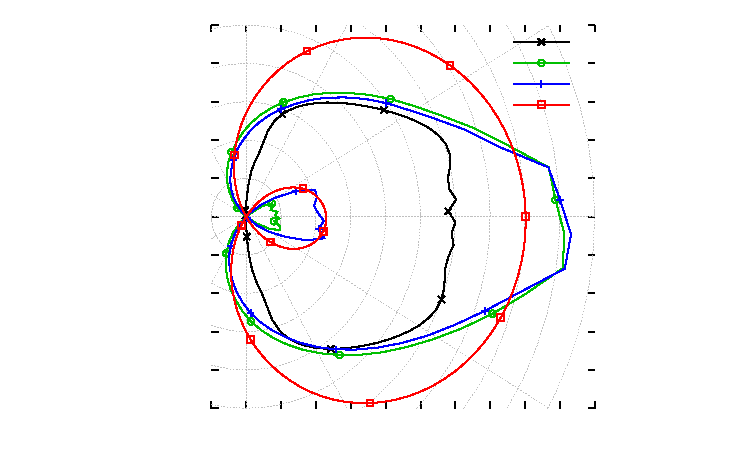
\includegraphics{/Users/seth/_thesis/figures/crashpipe2b/intens-x1-t1/intensity-x1-t1.pdf}}%
    \gplfronttext
  \end{picture}%
\endgroup

  \hspace{-.5in}
  \caption{Scalar flux along the centerline of the channel with an isotropic
  boundary condition at $y=0$.}
  \label{fig:isotropic}
\end{figure}

% A visualization of the angular flux for each method (replacing Monte Carlo with
% an \SN\ solution), Fig.~\ref{fig:isotropicAngular}, helps explain the accuracy
% of the AD method and the difference between the reflecting and white boundary
% treatments. Even though AD cannot exactly model the peak of freely streaming
% photons in the channel (which the \SN\ angular flux shows at $\theta=3\pi/2$),
% it accurately approximates the angular flux shape driven by scattering from the
% diffusive region (the lobes on the left and right).
% The linear-in-angle diffusion approximation cannot represent any of these
% features.  

% \begin{figure}[htb!]
%  \centering
%  \hspace{-.5in}
%  % GNUPLOT: LaTeX picture with Postscript
\begingroup
  \makeatletter
  \providecommand\color[2][]{%
    \GenericError{(gnuplot) \space\space\space\@spaces}{%
      Package color not loaded in conjunction with
      terminal option `colourtext'%
    }{See the gnuplot documentation for explanation.%
    }{Either use 'blacktext' in gnuplot or load the package
      color.sty in LaTeX.}%
    \renewcommand\color[2][]{}%
  }%
  \providecommand\includegraphics[2][]{%
    \GenericError{(gnuplot) \space\space\space\@spaces}{%
      Package graphicx or graphics not loaded%
    }{See the gnuplot documentation for explanation.%
    }{The gnuplot epslatex terminal needs graphicx.sty or graphics.sty.}%
    \renewcommand\includegraphics[2][]{}%
  }%
  \providecommand\rotatebox[2]{#2}%
  \@ifundefined{ifGPcolor}{%
    \newif\ifGPcolor
    \GPcolortrue
  }{}%
  \@ifundefined{ifGPblacktext}{%
    \newif\ifGPblacktext
    \GPblacktexttrue
  }{}%
  % define a \g@addto@macro without @ in the name:
  \let\gplgaddtomacro\g@addto@macro
  % define empty templates for all commands taking text:
  \gdef\gplbacktext{}%
  \gdef\gplfronttext{}%
  \makeatother
  \ifGPblacktext
    % no textcolor at all
    \def\colorrgb#1{}%
    \def\colorgray#1{}%
  \else
    % gray or color?
    \ifGPcolor
      \def\colorrgb#1{\color[rgb]{#1}}%
      \def\colorgray#1{\color[gray]{#1}}%
      \expandafter\def\csname LTw\endcsname{\color{white}}%
      \expandafter\def\csname LTb\endcsname{\color{black}}%
      \expandafter\def\csname LTa\endcsname{\color{black}}%
      \expandafter\def\csname LT0\endcsname{\color[rgb]{1,0,0}}%
      \expandafter\def\csname LT1\endcsname{\color[rgb]{0,1,0}}%
      \expandafter\def\csname LT2\endcsname{\color[rgb]{0,0,1}}%
      \expandafter\def\csname LT3\endcsname{\color[rgb]{1,0,1}}%
      \expandafter\def\csname LT4\endcsname{\color[rgb]{0,1,1}}%
      \expandafter\def\csname LT5\endcsname{\color[rgb]{1,1,0}}%
      \expandafter\def\csname LT6\endcsname{\color[rgb]{0,0,0}}%
      \expandafter\def\csname LT7\endcsname{\color[rgb]{1,0.3,0}}%
      \expandafter\def\csname LT8\endcsname{\color[rgb]{0.5,0.5,0.5}}%
    \else
      % gray
      \def\colorrgb#1{\color{black}}%
      \def\colorgray#1{\color[gray]{#1}}%
      \expandafter\def\csname LTw\endcsname{\color{white}}%
      \expandafter\def\csname LTb\endcsname{\color{black}}%
      \expandafter\def\csname LTa\endcsname{\color{black}}%
      \expandafter\def\csname LT0\endcsname{\color{black}}%
      \expandafter\def\csname LT1\endcsname{\color{black}}%
      \expandafter\def\csname LT2\endcsname{\color{black}}%
      \expandafter\def\csname LT3\endcsname{\color{black}}%
      \expandafter\def\csname LT4\endcsname{\color{black}}%
      \expandafter\def\csname LT5\endcsname{\color{black}}%
      \expandafter\def\csname LT6\endcsname{\color{black}}%
      \expandafter\def\csname LT7\endcsname{\color{black}}%
      \expandafter\def\csname LT8\endcsname{\color{black}}%
    \fi
  \fi
  \setlength{\unitlength}{0.0500bp}%
  \begin{picture}(7200.00,4320.00)%
    \gplgaddtomacro\gplbacktext{%
      \csname LTb\endcsname%
      \put(1910,400){\makebox(0,0)[r]{\strut{} 0.1}}%
      \put(1910,768){\makebox(0,0)[r]{\strut{} 0.08}}%
      \put(1910,1136){\makebox(0,0)[r]{\strut{} 0.06}}%
      \put(1910,1504){\makebox(0,0)[r]{\strut{} 0.04}}%
      \put(1910,1872){\makebox(0,0)[r]{\strut{} 0.02}}%
      \put(1910,2240){\makebox(0,0)[r]{\strut{} 0}}%
      \put(1910,2607){\makebox(0,0)[r]{\strut{} 0.02}}%
      \put(1910,2975){\makebox(0,0)[r]{\strut{} 0.04}}%
      \put(1910,3343){\makebox(0,0)[r]{\strut{} 0.06}}%
      \put(1910,3711){\makebox(0,0)[r]{\strut{} 0.08}}%
      \put(1910,4079){\makebox(0,0)[r]{\strut{} 0.1}}%
      \csname LTb\endcsname%
      \put(2030,200){\makebox(0,0){\strut{} 0.02}}%
      \csname LTb\endcsname%
      \put(2364,200){\makebox(0,0){\strut{} 0}}%
      \csname LTb\endcsname%
      \put(2699,200){\makebox(0,0){\strut{} 0.02}}%
      \csname LTb\endcsname%
      \put(3033,200){\makebox(0,0){\strut{} 0.04}}%
      \csname LTb\endcsname%
      \put(3368,200){\makebox(0,0){\strut{} 0.06}}%
      \csname LTb\endcsname%
      \put(3702,200){\makebox(0,0){\strut{} 0.08}}%
      \csname LTb\endcsname%
      \put(4037,200){\makebox(0,0){\strut{} 0.1}}%
      \csname LTb\endcsname%
      \put(4371,200){\makebox(0,0){\strut{} 0.12}}%
      \csname LTb\endcsname%
      \put(4706,200){\makebox(0,0){\strut{} 0.14}}%
      \csname LTb\endcsname%
      \put(5040,200){\makebox(0,0){\strut{} 0.16}}%
      \csname LTb\endcsname%
      \put(5375,200){\makebox(0,0){\strut{} 0.18}}%
      \csname LTb\endcsname%
      \put(5709,200){\makebox(0,0){\strut{} 0.2}}%
      \csname LTb\endcsname%
      \put(1330,2239){\rotatebox{-270}{\makebox(0,0){\strut{}x1 center $(1.01,3.5)$}}}%
    }%
    \gplgaddtomacro\gplfronttext{%
      \csname LTb\endcsname%
      \put(4806,3916){\makebox(0,0)[r]{\strut{}S$_{128}$}}%
      \csname LTb\endcsname%
      \put(4806,3716){\makebox(0,0)[r]{\strut{}FLAD$_{64}$}}%
      \csname LTb\endcsname%
      \put(4806,3516){\makebox(0,0)[r]{\strut{}AD$_{64}$}}%
      \csname LTb\endcsname%
      \put(4806,3316){\makebox(0,0)[r]{\strut{}FLD}}%
    }%
    \gplbacktext
    \put(0,0){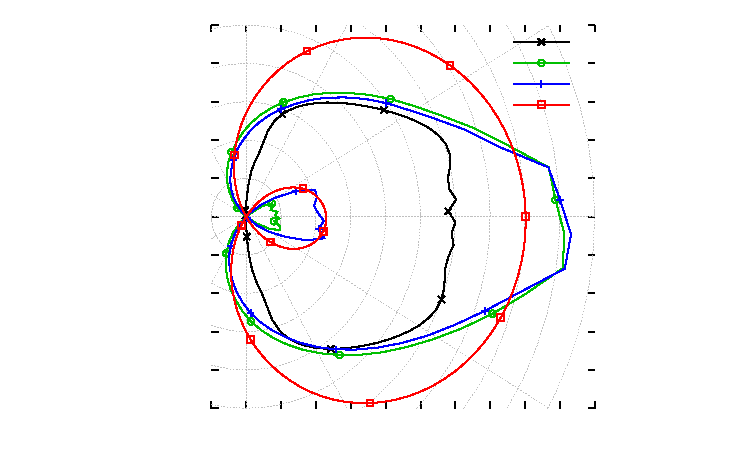
\includegraphics{/Users/seth/_thesis/figures/crashpipe2b/intens-x1-t1/intensity-x1-t1.pdf}}%
    \gplfronttext
  \end{picture}%
\endgroup

%  \hspace{-.5in}
%  \caption{Angular flux $\psi(2.5, 1., \theta)$, in the centerline of the
%  channel one unit from the boundary.}
%  \label{fig:isotropicAngular}
% \end{figure}

% The shape around $\theta=\pi/2$ gives insight into why the white boundary
% performs better in this problem: a reflecting boundary produces a peak in $f$
% along the channel, but a white boundary gives a more isotropic shape near that
% range, better matching the incident isotropic boundary condition. This suggests
% that the qualitatively best way to satisfy Eq.~\eqref{eq:zetaCondition} may be
% to have $\zeta$ take the shape of the true boundary condition.

A close examination of the numerical solutions gives some insight into these
results.  AD does not exactly model the peak of freely streaming
photons in the channel, but it does accurately approximate the angular flux
shape driven by scattering from the diffusive regions along the edge of the
channel. 
The standard linear-in-angle diffusion approximation does not accurately
represent these
features.  Also, a reflecting boundary for $f$ produces a peak in $f$
along the channel, but a white boundary condition gives a more isotropic shape,
better matching the incident isotropic boundary condition. This suggests that a
more accurate way to satisfy Eq.~\eqref{eq:zetaCondition} may be to have
$\zeta$ take the shape of the true boundary condition. This wil be examined in
future work. 


%%%%%%%%%%%%%%%%%%%%%%%%%%%%%%%%%%%%%%%%%%%%%%%%%%%%%%%%%%%%%%%%%%%%%%%%%%%%%%%%
\section{Conclusions}

We have presented a new derivation of the anisotropic diffusion (AD)
approximation to
the transport equation, yielding both the previously-known AD equation and new
boundary conditions for this equation. The AD method requires that a
purely-absorbing transport problem be solved to determine the anisotropic
diffusion coefficients. Because of this, the AD approximation is more costly
than standard diffusion, but much less costly than a transport simulation
(Monte Carlo or deterministic). Numerical testing of a problem with two
diffusive regions bordering an optically thin channel, driven by a surface
source, show that the AD method is much more accurate than standard diffusion,
with results comparable to Monte Carlo. 

%%%%%%%%%%%%%%%%%%%%%%%%%%%%%%%%%%%%%%%%%%%%%%%%%%%%%%%%%%%%%%%%%%%%%%%%%%%%%%%%
\section{Acknowledgments}
This material is based upon work supported under a Department of Energy Nuclear
Energy University Programs Graduate Fellowship.

%%%%%%%%%%%%%%%%%%%%%%%%%%%%%%%%%%%%%%%%%%%%%%%%%%%%%%%%%%%%%%%%%%%%%%%%%%%%%%%%
\bibliographystyle{ans}
\bibliography{../SRJall}
\end{document}

